\documentclass{beamer}
\usepackage{tikz}
\usepackage[all]{xy}
\usepackage{amsmath,amssymb}
\usepackage{hyperref}
\usepackage{graphicx}
\usepackage[noend]{algcompatible}
\usepackage{multirow}

\DeclareMathOperator*{\argmin}{arg\,min}
\DeclareMathOperator*{\Lik}{Lik}
\DeclareMathOperator*{\PoissonLoss}{PoissonLoss}
\DeclareMathOperator*{\Peaks}{Peaks}
\DeclareMathOperator*{\Segments}{Segments}
\DeclareMathOperator*{\argmax}{arg\,max}
\DeclareMathOperator*{\maximize}{maximize}
\DeclareMathOperator*{\minimize}{minimize}
\newcommand{\sign}{\operatorname{sign}}
\newcommand{\RR}{\mathbb R}
\newcommand{\ZZ}{\mathbb Z}
\newcommand{\NN}{\mathbb N}
\newcommand{\z}{$z = 2, 4, 3, 5, 1$} 

\newcommand{\algo}[1]{\textcolor{#1}{#1}}
\definecolor{PDPA}{HTML}{66C2A5}
\definecolor{CDPA}{HTML}{FC8D62}
\definecolor{GPDPA}{HTML}{4D4D4D}

% Set transparency of non-highlighted sections in the table of
% contents slide.
\setbeamertemplate{section in toc shaded}[default][100]
\AtBeginSection[]
{
  \setbeamercolor{section in toc}{fg=red} 
  \setbeamercolor{section in toc shaded}{fg=black} 
  \begin{frame}
    \tableofcontents[currentsection]
  \end{frame}
}

\begin{document}

\title{Optimizing ROC Curves with a Sort-Based Surrogate Loss for Binary Classification and Changepoint Detection, arXiv:2107.01285}

\author{
  Toby Dylan Hocking --- toby.hocking@nau.edu\\ 
  joint work with my student Jonathan Hillman\\
  Machine Learning Research Lab --- \url{http://ml.nau.edu}\\
  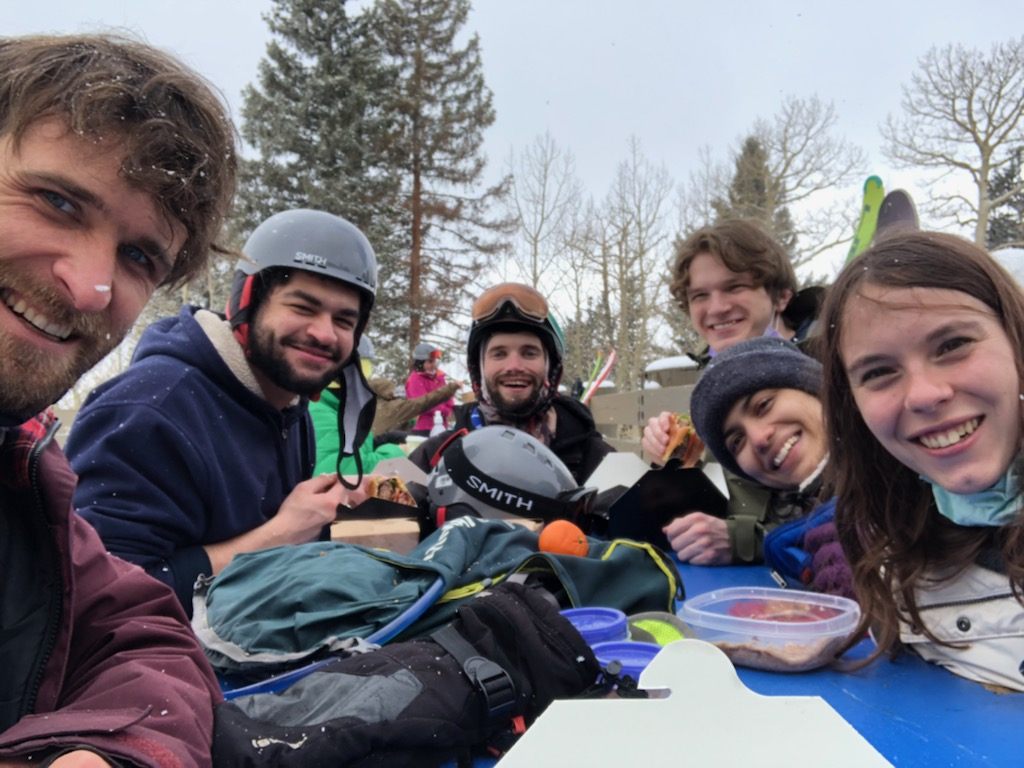
\includegraphics[height=3.5cm]{2021-03-lab-ski-lunch} \\
  Come to SICCS! Graduate Research Assistantships available!
}

\date{}

\maketitle 

\section{Problem Setting and Related Work}

\begin{frame}
  \frametitle{Problem: unsupervised changepoint detection}
  \begin{itemize}
  \item We are given a data sequence $z_1,\dots,z_T$ measured at $T$
    points over time/space.
  \item Ex: DNA copy number data for cancer diagnosis, $z_t\in\mathbb R$.
  \item The penalized changepoint problem is
$$\argmin_{u_1,\dots,u_T\in\mathbb R} \sum_{t=1}^T (u_t - z_t)^2 + \lambda\sum_{t=2}^T I[u_{t-1} \neq u_t].$$
  \end{itemize}

  \parbox{0.6\textwidth}{
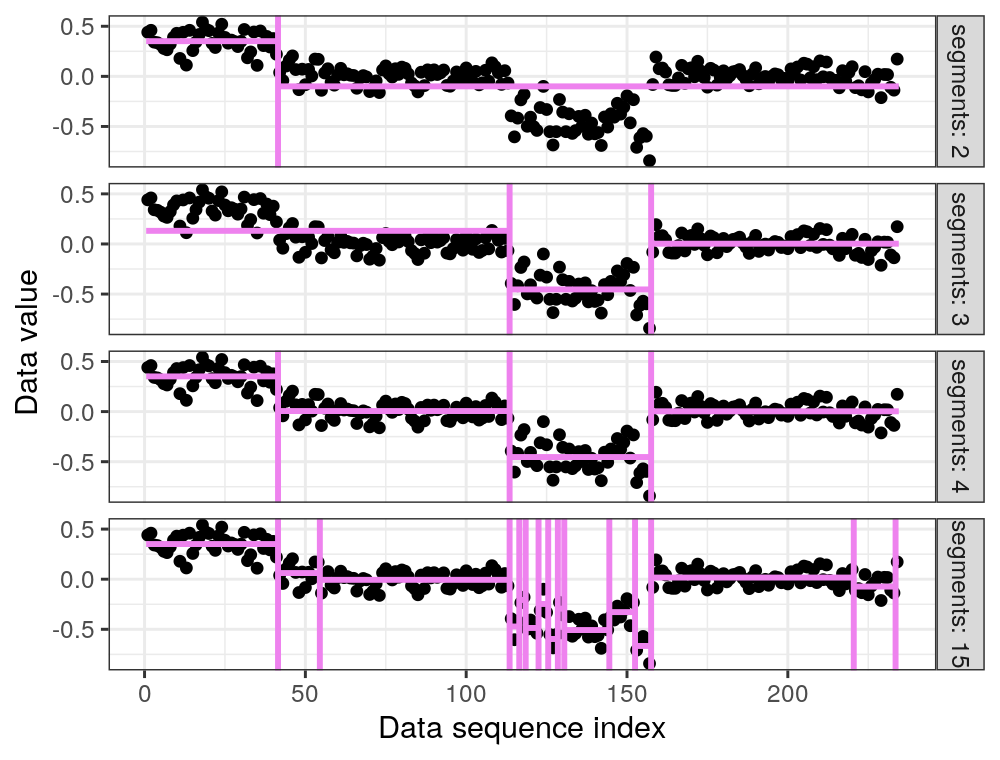
\includegraphics[width=0.6\textwidth]{figure-fn-not-monotonic-no-labels}
}
\parbox{0.3\textwidth}{
  Larger penalty $\lambda$ results in fewer changes/segments.

  \vskip 0.5in

  Smaller penalty $\lambda$ results in more changes/segments.
}

\end{frame}


\begin{frame}
  \frametitle{Problem: weakly supervised changepoint detection}
  \begin{itemize}
  \item We are given a data sequence $\mathbf z$ with labeled regions
    $L$.
  \item We compute features $\mathbf x=\phi(\mathbf z)\in\mathbf R^p$
    and want to learn a function $f(\mathbf x)=-\log\lambda\in\mathbf R$ that minimizes label
    error.
  \end{itemize}

  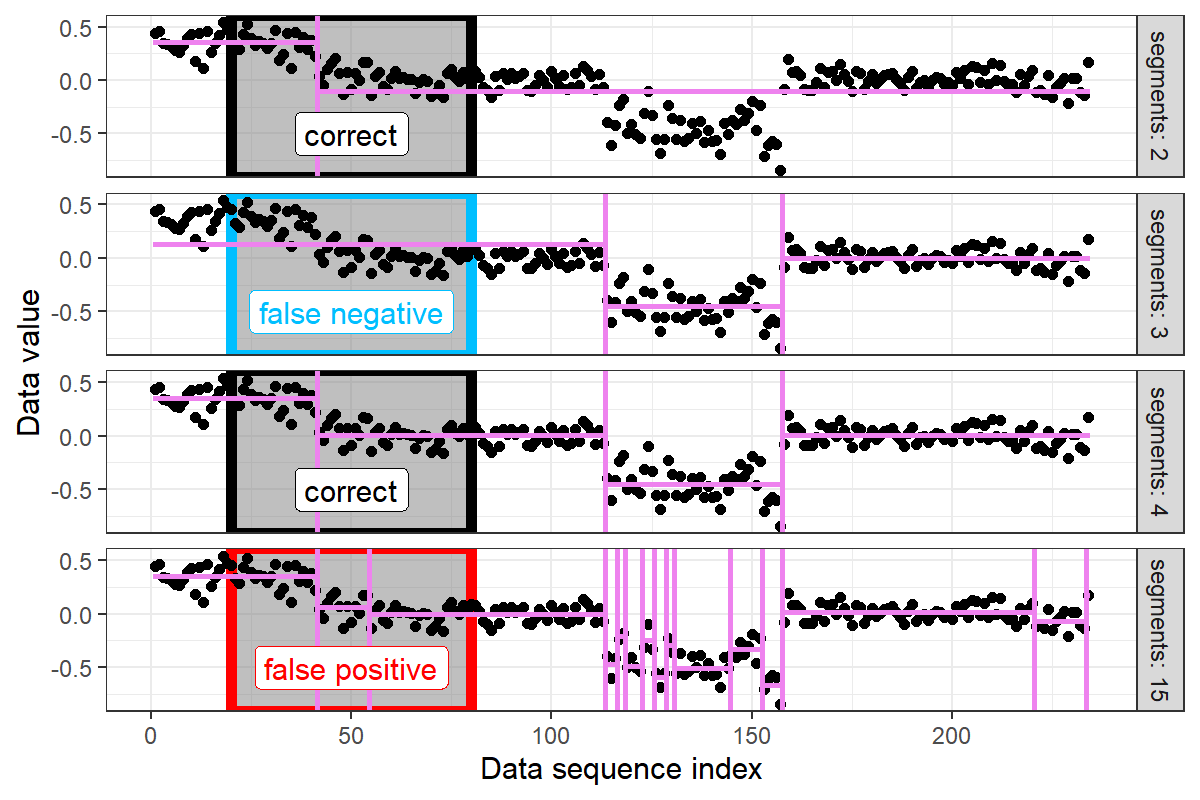
\includegraphics[width=0.7\textwidth]{figure-fn-not-monotonic}

\end{frame}

\begin{frame}
  \frametitle{Problem: supervised binary classification}
  
  \begin{itemize}
  \item Given pairs of inputs $\mathbf x\in\mathbb R^p$ and outputs
    $y\in\{0,1\}$ can we learn $f(\mathbf x)= y$?
  \item Example: email, $\mathbf x =$bag of words, $y=$spam or not.
  \item Example: images. Jones {\it et al.} PNAS 2009. 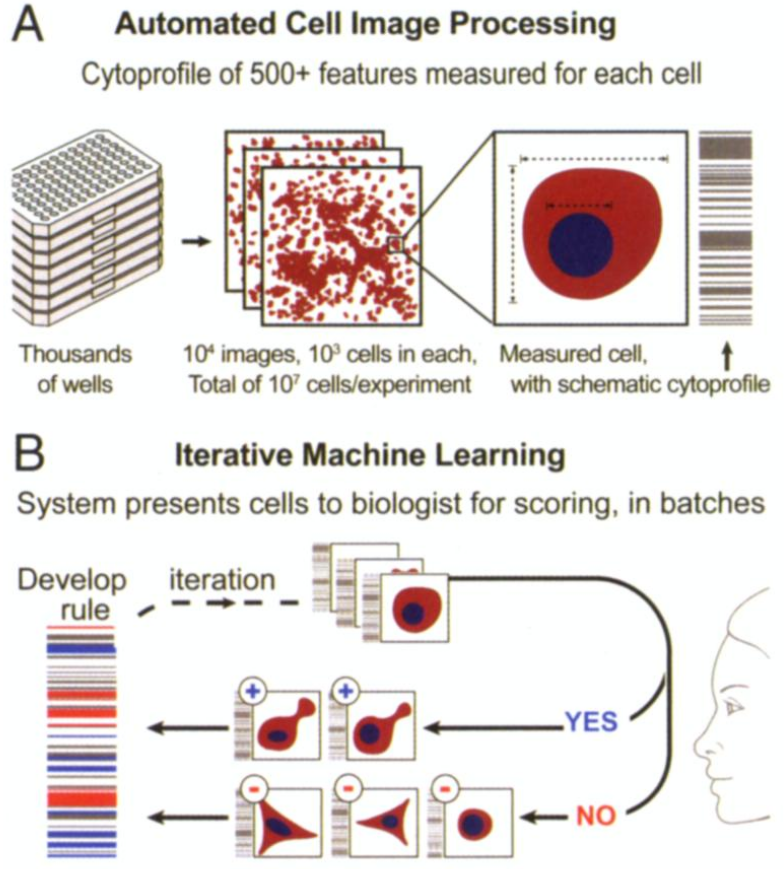
\includegraphics[width=2in]{cellprofiler} 
  \end{itemize} 

\end{frame}

\begin{frame}
  \frametitle{Receiver Operating Characteristic (ROC) curve}

  \begin{itemize}
  \item ROC curve is plot of x=FPR, y=TPR. 
  \item Best point in ROC space is upper left (0\% FPR, 100\% TPR).
  \item Binary classification algo gives predictions.
    $[\hat y_1,\hat y_2,\hat y_3,\hat y_4]$.
  \item Each point on the ROC curve is the FPR/TPR if you add some
  constant $c$ to the predictions,
  $[\hat y_1+c,\hat y_2+c,\hat y_3+c,\hat y_4+c]$.
  \item Maximizing Area Under the ROC curve (AUC) is a common
    objective for binary classification, especially for imbalanced
    data (example: 99\% positive, 1\% negative labels).
  \end{itemize} 
  
  \parbox{1.5in}{
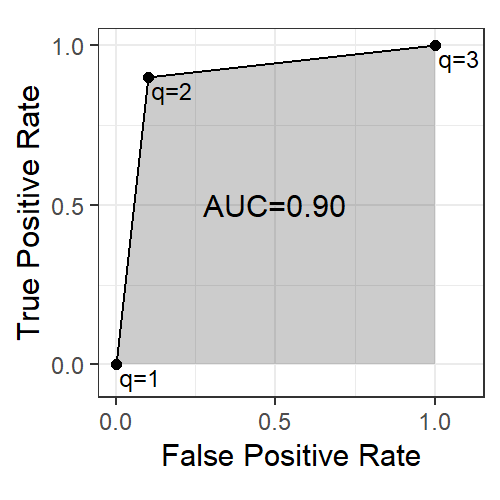
\includegraphics[width=1.5in]{figure-more-than-one-less-auc}
}
\parbox{2.5in}{
In binary classification, ROC curve is monotonic increasing.
  \begin{itemize}
  \item AUC=1 best.
  \item AUC=0.5 for constant prediction (usually worst).
  \end{itemize}
}

\end{frame}

\begin{frame}
  \frametitle{Area Under ROC curve, synthetic example}

\begin{itemize}
  \item label = [1,0,0,...,1,1,0] (20 labels, 10 positive, 10 negative).
  \item predictions = [-4, -4, -4, ..., -2, -2, -2].
  \item No constant added $c=0$, $q=1$, everything predicted negative,
    so no false positives, but no true positives.
% > WeightedROC::WeightedAUC(WeightedROC::WeightedROC(c(-8,-8,-5,-5), c(1,0,1,0), c(1,9,9,1)))
% [1] 0.9
\item Add $c=3 \Rightarrow$ [-1, -1, -1, ..., 1, 1, 1], 1 FP and
  9 TP, $q=2$.
\item  Add $c=5 \Rightarrow$ [1, 1, 1, ..., 3, 3, 3], all FP and TP, $q=3$.
  \end{itemize}

  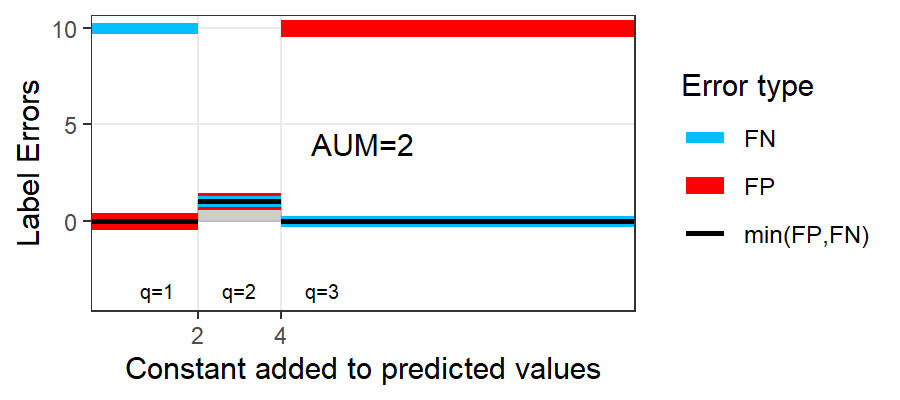
\includegraphics[height=1.5in]{figure-more-than-one-less-aum}
  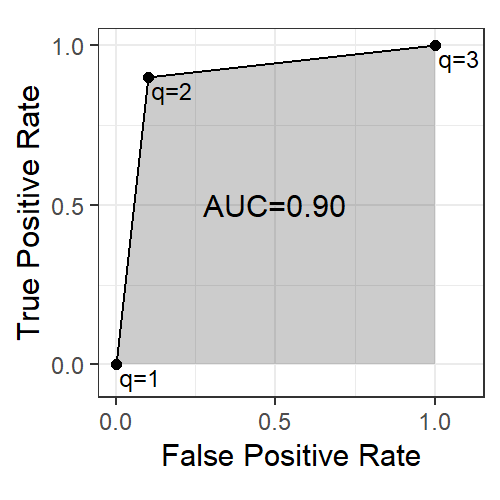
\includegraphics[height=1.5in]{figure-more-than-one-less-auc}

\end{frame}


\section{Proposed algorithm}

\begin{frame}
  \frametitle{Looping ROC curve, simple synthetic example}

If ROC curve has loops, AUC can be greater than one.

  \begin{itemize}
  \item Dark grey area double counted.
  \item Red area negative counted.
  \item Do we want to maximize AUC?
  \item Minimize Area Under Min (AUM) instead, which encourages ROC
    points in upper left.
  \end{itemize}

  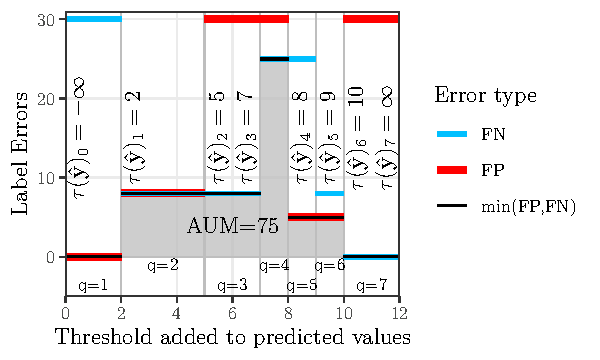
\includegraphics[height=1.5in]{figure-more-than-one-more-aum}
  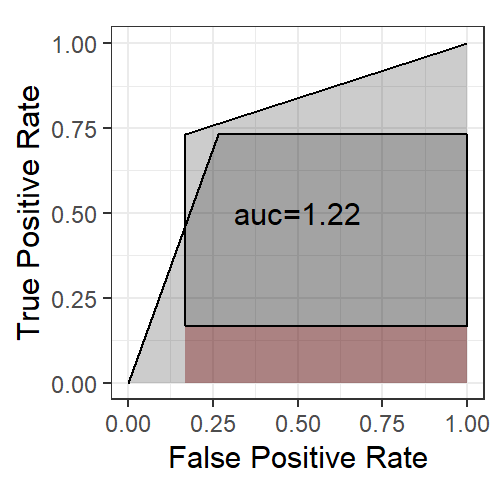
\includegraphics[height=1.5in]{figure-more-than-one-more-auc}

\end{frame}

\begin{frame}
  \frametitle{Real data example with non-monotonic label error}

  ROC curve loops result from non-monotonic FP/FN functions, but do
  these occur in real data? Yes, in supervised changepoint
  problems.
  
  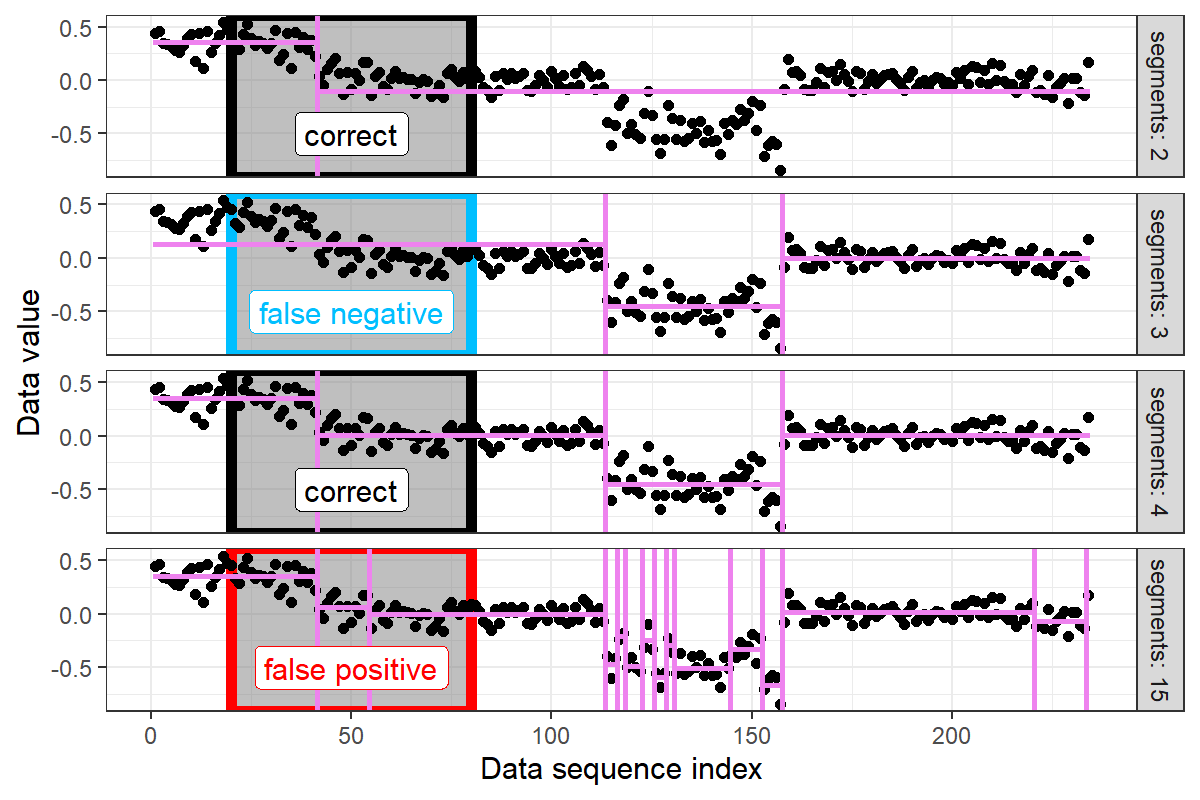
\includegraphics[width=0.49\textwidth]{figure-fn-not-monotonic}
  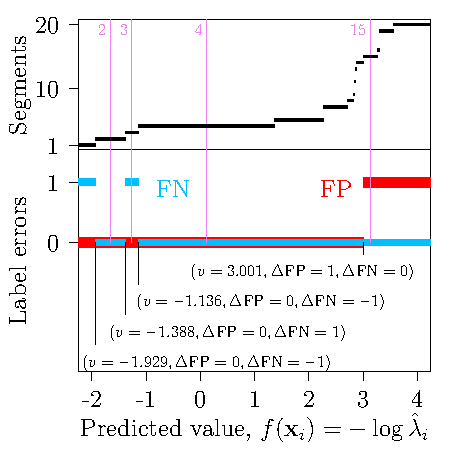
\includegraphics[width=0.49\textwidth]{figure-fn-not-monotonic-error-standAlone}

  Optimal changepoint model may have non-monotonic error (for example
  FN), because changepoints at model size $s$ may not be present in
  model $s+1$.

\end{frame}

\begin{frame}
  \frametitle{Real data example with AUC greater than one}

  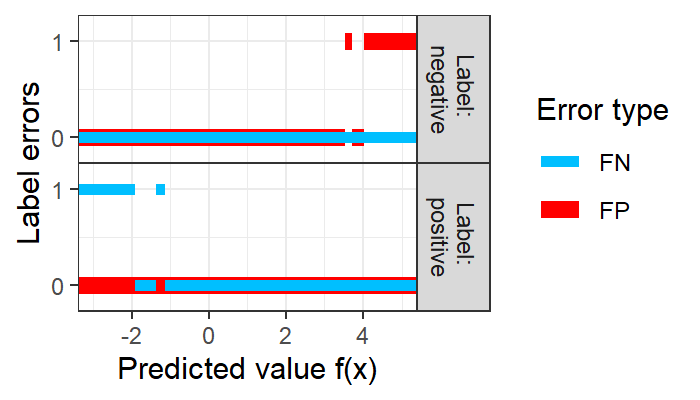
\includegraphics[height=1.3in]{figure-aum-convexity-profiles}
  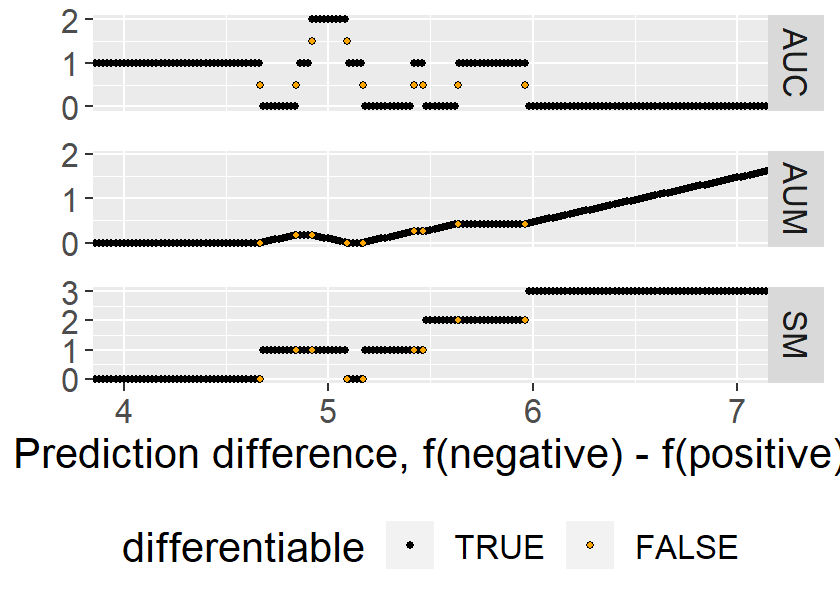
\includegraphics[height=1.3in]{figure-aum-convexity}

  \begin{itemize}
  \item $n=2$ labeled changepoint problems.
  \item AUC=2 when prediction difference=5.
  \item AUM=0 implies AUC=1.
  \item AUM is convex relaxation of non-convex Sum of Min (SM).
  \item AUM is differentiable almost everywhere.
  \item Main new idea: compute the gradient of this function and use
    it for learning.
  \end{itemize}

\end{frame}




\begin{frame}
  \frametitle{Algorithm inputs: predictions and label error functions}

  \begin{itemize}
  \item Each observation $i\in\{1,\dots,n\}$ has a predicted value
    $\hat y_i\in\mathbb R$.
  \item Breakpoints
  $b\in\{1,\dots, B\}$ used to represent label error via tuple
  $(v_b, \Delta\text{FP}_b, \Delta\text{FN}_b, \mathcal I_b)$.
\item There are changes $\Delta\text{FP}_b, \Delta\text{FN}_b$ at
  predicted value $v_b\in\mathbb R$ in error function
  $\mathcal I_b\in\{1,\dots,n\}$.
  \end{itemize}

  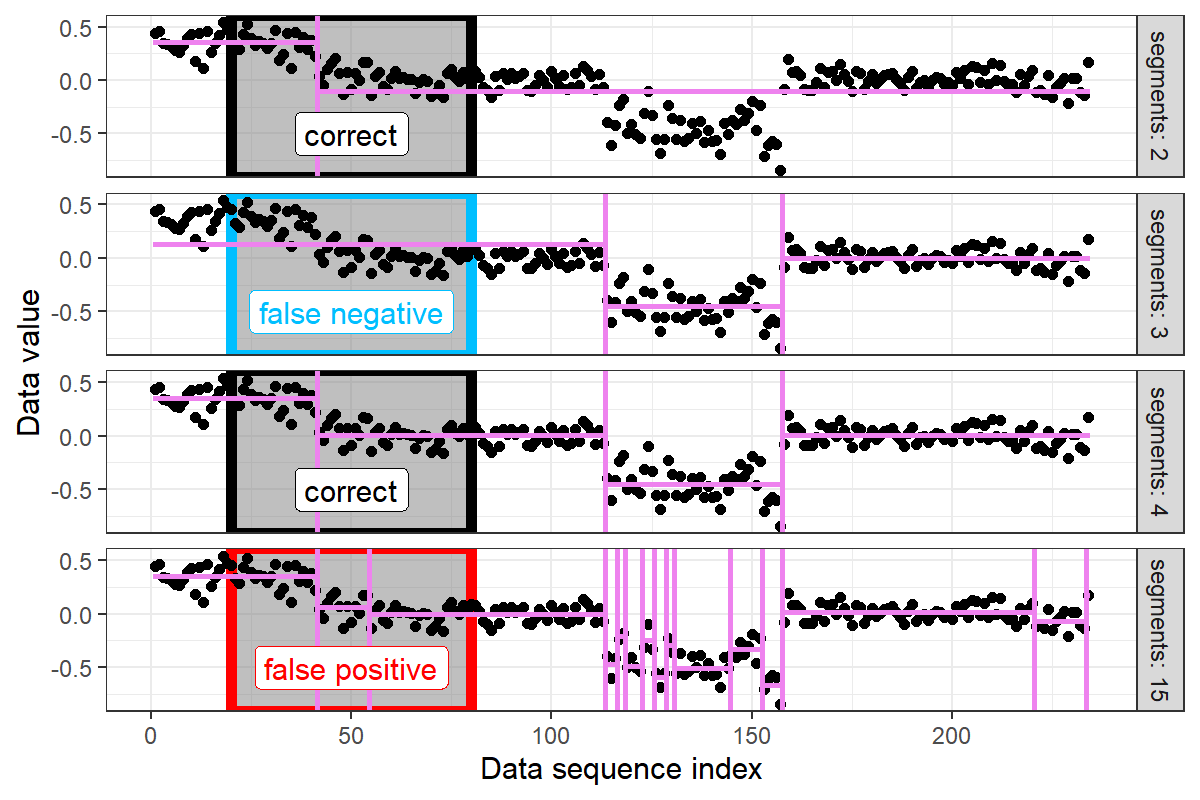
\includegraphics[width=0.49\textwidth]{figure-fn-not-monotonic}
  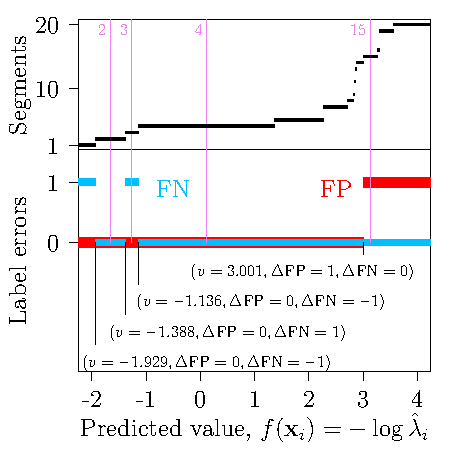
\includegraphics[width=0.49\textwidth]{figure-fn-not-monotonic-error-standAlone}

\end{frame}

\begin{frame}
  \frametitle{Algorithm computes total FP and FN for each threshold/constant added to predicted values}
  \begin{itemize}
  \item Breakpoint threshold,
    $t_b= v_b - \hat y_{\mathcal I_b}=\tau(\mathbf{\hat y})_q$ for
    some $q$.
  \item Total error before/after each breakpoint can be computed via
    sort and modified cumsum:
  \end{itemize}
\begin{eqnarray*}
  \underline{\text{FP}}_b &=& \sum_{j: t_j < t_b} \Delta\text{FP}_j,\ 
  \overline{\text{FP}}_b = \sum_{j: t_j \leq t_b} \Delta\text{FP}_j, \\
  \underline{\text{FN}}_b &=& \sum_{j: t_j \geq t_b} - \Delta\text{FN}_j,\ 
  \overline{\text{FN}}_b = \sum_{j: t_j > t_b} - \Delta\text{FN}_j.
\end{eqnarray*}

  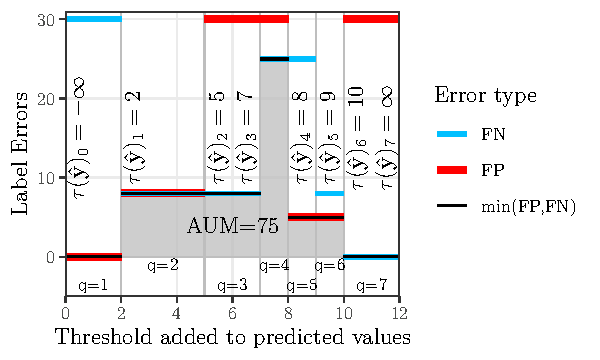
\includegraphics[height=1.5in]{figure-more-than-one-more-aum}

\end{frame}

\begin{frame}
  \frametitle{Algorithm computes two directional derivatives }

  \begin{itemize}
  \item Gradient only defined when function is differentiable, but AUM
    is not everywhere (see below).
  \item Directional derivatives defined everywhere.
  \end{itemize}
% \begin{theorem}
% \label{thm:directional-derivs}
% The AUM directional derivatives for a particular example
% $i\in\{1,\dots,n\}$ can be computed using the following equations.
% \end{theorem}
\begin{eqnarray*}
  &&\nabla_{\mathbf v(-1,i)} \text{AUM}(\mathbf{\hat y}) = \\
  &&\sum_{b: \mathcal I_b = i}
  \min\{
  \overline{\text{FP}}_b , 
  \overline{\text{FN}}_b 
  \}
  -
  \min\{
  \overline{\text{FP}}_b - \Delta\text{FP}_b, 
  \overline{\text{FN}}_b - \Delta\text{FN}_b
  \},\\
  &&\nabla_{\mathbf v(1,i)} \text{AUM}(\mathbf{\hat y}) = \\
  &&\sum_{b: \mathcal I_b = i}
  \min\{
  \underline{\text{FP}}_b + \Delta\text{FP}_b, 
  \underline{\text{FN}}_b + \Delta\text{FN}_b
  \}
  -
  \min\{
  \underline{\text{FP}}_b , 
  \underline{\text{FN}}_b 
     \}.
\end{eqnarray*}  

  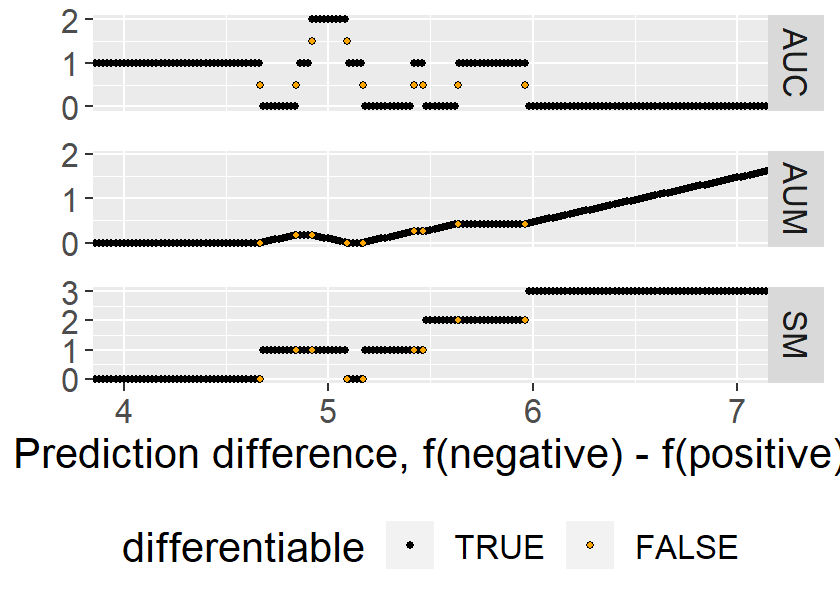
\includegraphics[height=1.6in]{figure-aum-convexity}

\end{frame}


\begin{frame}
  \frametitle{Proposed algorithm uses sort to compute AUM and directional derivatives}

\small
\begin{algorithmic}[1]
  \STATE {\bfseries Input:} 
  Predictions $\mathbf{\hat y}\in\mathbb R^n$, 
  breakpoints in error functions $v_b,\Delta\text{FP}_b,\Delta\text{FN}_b,\mathcal I_b$ for all $b\in\{1,\dots,B\}$.
  \STATE Zero the $\text{AUM}\in\mathbb R$ and directional derivatives $\mathbf D\in\mathbb R^{n\times 2}$.\label{line:init-zero}
  \STATE $t_b\gets v_b - \hat y_{\mathcal I_b}$ for all $b$.\label{line:compute-thresh}
  \STATE $s_1,\dots,s_B\gets \textsc{SortedIndices}(t_1,\dots,t_B).$\label{line:sorted-indices}
  \STATE Compute $\underline{\text{FP}}_b,\overline{\text{FP}}_b,\underline{\text{FN}}_b,\overline{\text{FN}}_b$ for all $b$ using $s_1,\dots,s_B$.
  \FOR{$b\in\{2,\dots,B\}$}\label{line:for-intervals}
  \STATE $\text{AUM} \text{ += } (t_{s_b} - t_{s_{b-1}}) \min\{\underline{\text{FP}}_b, \overline{\text{FN}}_b\} $.\label{line:AUM}
  \ENDFOR
  \FOR{$b\in\{1,\dots,B\}$}\label{line:for-breakpoints}
  \STATE\label{line:D_lo} $\mathbf D_{\mathcal I_b,1} \text{ += } \min\{
  \overline{\text{FP}}_b , 
  \overline{\text{FN}}_b 
  \}
  -
  \min\{
  \overline{\text{FP}}_b - \Delta\text{FP}_b, 
  \overline{\text{FN}}_b - \Delta\text{FN}_b
  \}$
  \STATE\label{line:D_hi} $\mathbf D_{\mathcal I_b,2} \text{ += } \min\{
  \underline{\text{FP}}_b + \Delta\text{FP}_b, 
  \underline{\text{FN}}_b + \Delta\text{FN}_b
  \}
  -
  \min\{
  \underline{\text{FP}}_b , 
  \underline{\text{FN}}_b 
  \}$
  \ENDFOR
  \STATE {\bfseries Output:} AUM and matrix $\mathbf D$ of directional derivatives.
\end{algorithmic}
\begin{itemize}
\item 
 Overall $O(B\log B)$ time due to sort.
\end{itemize}
  
\end{frame}
\section{Empirical results}

\begin{frame}
  \frametitle{Train set ROC curves for a real changepoint problem}

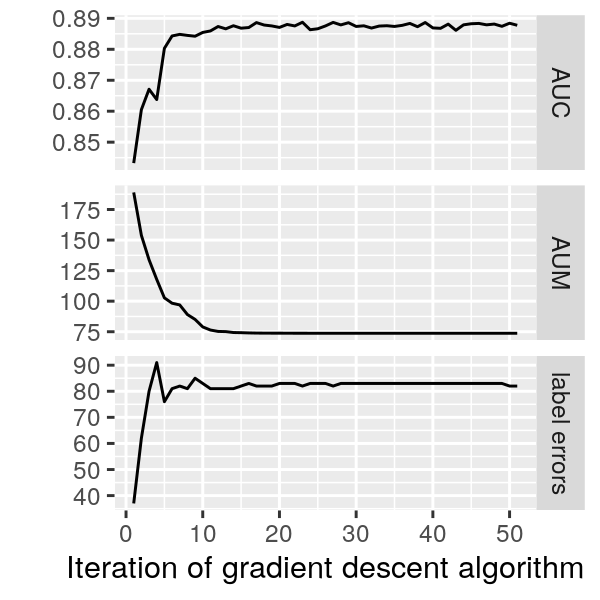
\includegraphics[height=3.7cm]{figure-aum-optimized-iterations.png}
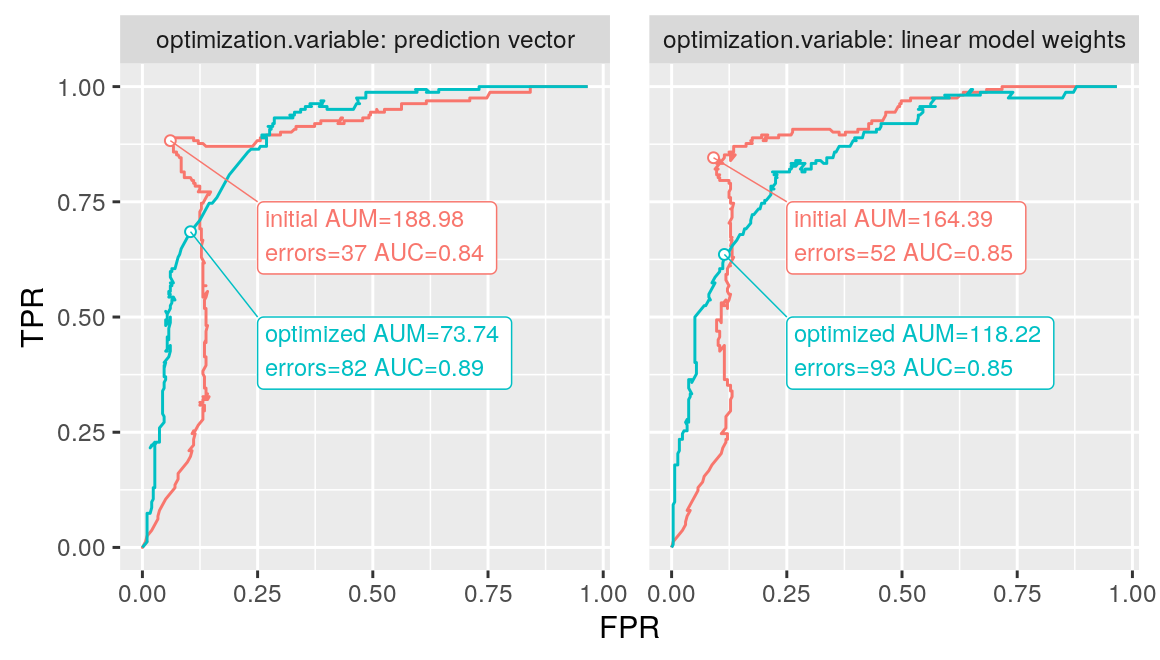
\includegraphics[height=3.7cm]{figure-aum-train-both.png}

\begin{itemize}
\item Left/middle: changepoint problem initialized to prediction vector with
  min label errors, gradient descent on prediction vector.
\item Right: linear model initialized by minimizing regularized convex
  loss (surrogate for label error), gradient descent on weight vector.
\end{itemize}

\end{frame}

\begin{frame}
  \frametitle{Learning algorithm results in better test AUC/AUM for changepoint problems}
    
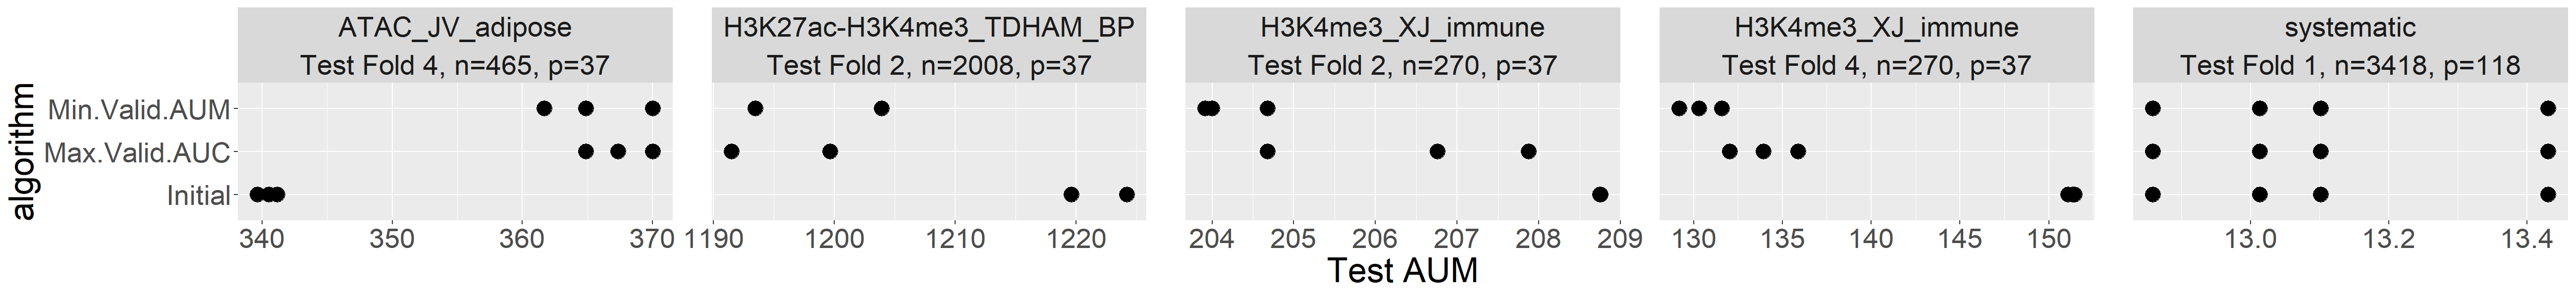
\includegraphics[width=\textwidth]{figure-test-aum-comparison.png}
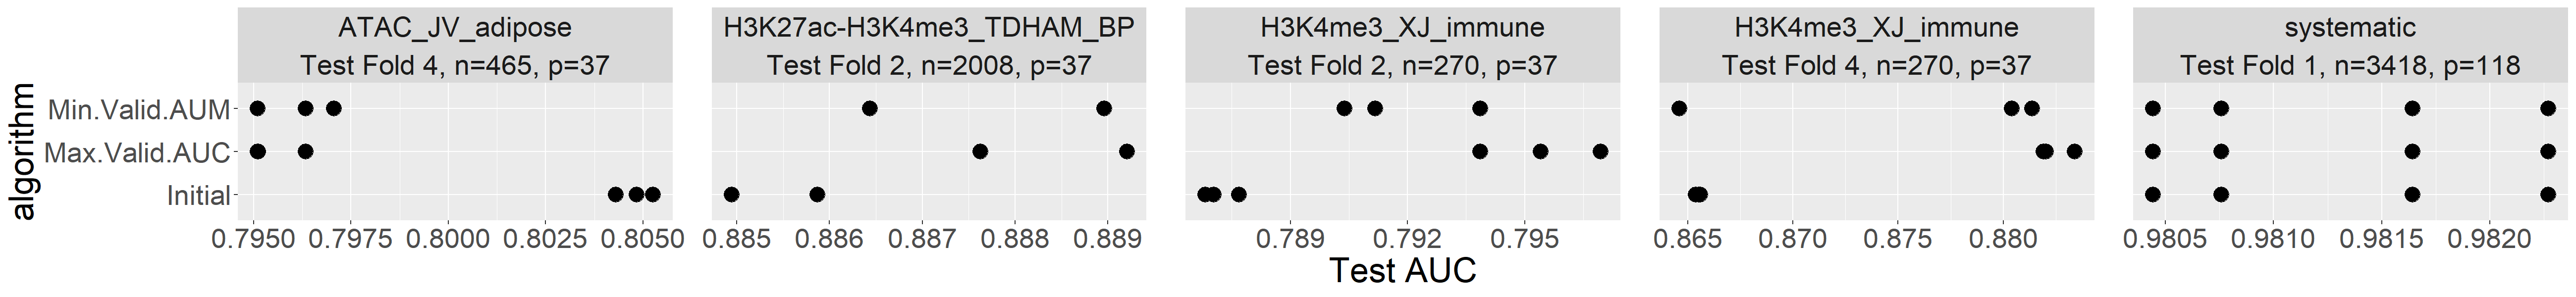
\includegraphics[width=\textwidth]{figure-test-auc-comparison.png}

\begin{itemize}
\item Five changepoint problems (panels from left to right).
\item Two evaluation metrics (AUM=top, AUC=bottom).
\item Three algorithms (Y axis), Initial=Min regularized convex loss
  (surrogate for label error), Min.Valid.AUM/Min.Valid.AUC=AUM
  gradient descent with early stopping regularization.
\end{itemize}

\end{frame}

\begin{frame}
  \frametitle{Standard logistic loss fails for highly imbalanced labels}

 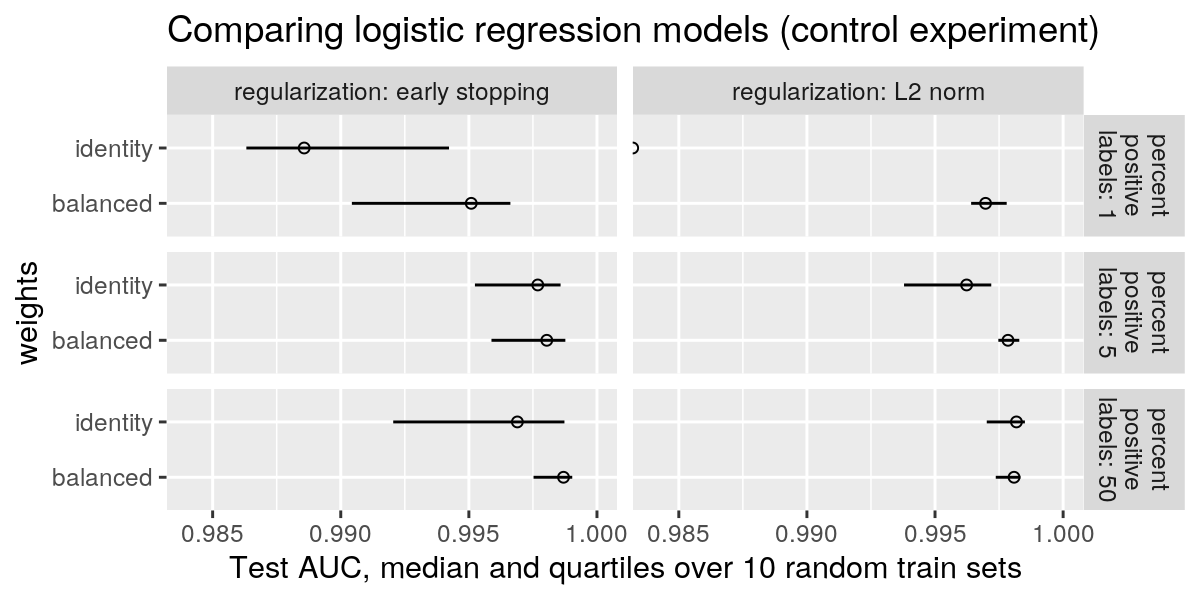
\includegraphics[width=\textwidth]{figure-unbalanced-grad-desc-logistic.png}

 \begin{itemize}
 \item Test set has 50\% positive, 50\% negative labels.
 \item Train set has variable class imbalance (panels top to
   bottom).
 \item Loss is $\ell[f(x_i), y_i]w_i$ with $w_i=1$ for identity
   weights, $w_i=1/N_{y_i}$ for balanced, ex: 1\% position means
   $w_i\in\{1/10,1/990\}$.
 \end{itemize}

\end{frame}


\begin{frame}
  \frametitle{Error rate loss is not as useful as error count loss}

 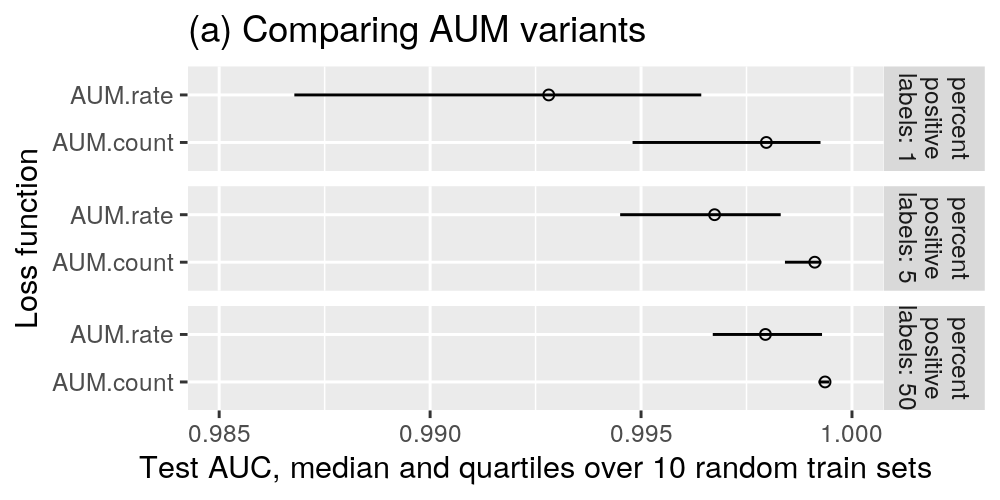
\includegraphics[width=\textwidth]{figure-unbalanced-grad-desc-aum.png}

 \begin{itemize}
 \item AUM.count is as described previously: error functions used to
   compute Min(FP,FN) are absolute label counts.
 \item AUM.rate is a variant which uses normalized error functions,
   Min(FPR,FNR).
 \item Both linear models with early stopping regularization.
 \end{itemize}

\end{frame}

\begin{frame}
  \frametitle{Learning algorithm competitive for unbalanced binary classification}

 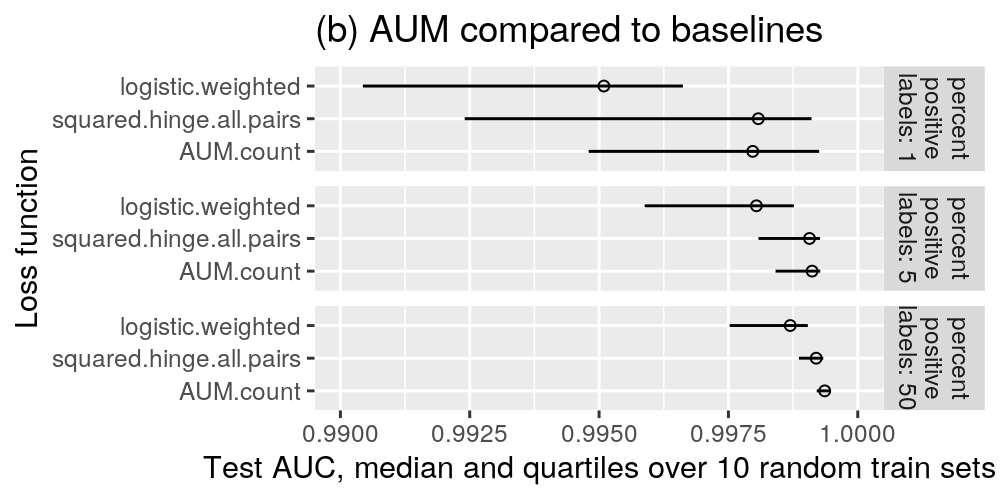
\includegraphics[width=\textwidth]{figure-unbalanced-grad-desc.png}

 \begin{itemize}
 \item Squared hinge all pairs is a classic/popular surrogate loss function
   for AUC optimization.
 \item All linear models with early stopping regularization.
 \end{itemize}

\end{frame}

\begin{frame}
  \frametitle{Comparable computation time to other loss functions}

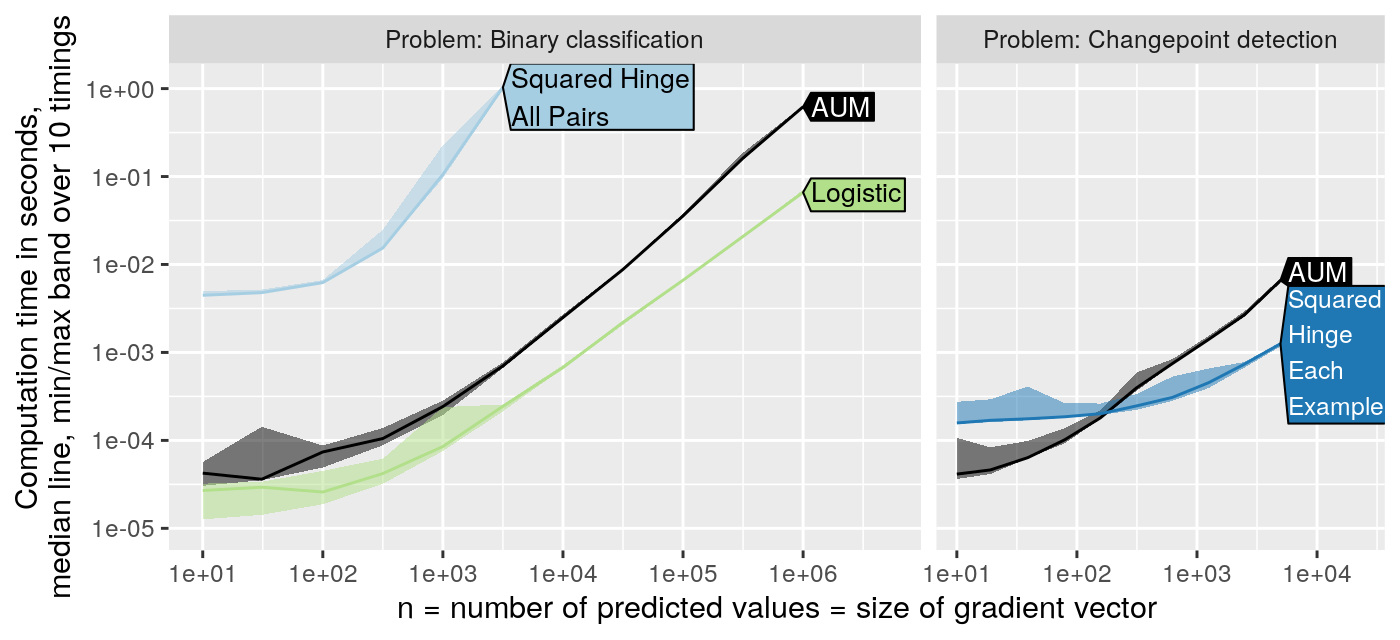
\includegraphics[width=\textwidth]{figure-aum-grad-speed-both.png}

\begin{itemize}
\item Logistic $O(n)$.
\item AUM $O(n\log n)$.
\item Squared Hinge All Pairs $O(n^2)$.
\item Squared Hinge Each Example $O(n)$.
\end{itemize}
  
\end{frame}

\section{Discussion and Conclusions}

\begin{frame}
  \frametitle{Conclusions, Pre-print arXiv:2107.01285}
  \begin{itemize}
  \item ROC curves are used to evaluate binary classification and
    changepoint detection algorithms.
  \item In changepoint detection there can be loops in ROC curves, so
    maximizing AUC may not be desirable.
  \item Instead we propose to minimize a new loss, AUM=Area
    Under Min(FP,FN).
  \item We propose new algorithm for efficient AUM and directional
    derivative computation.
  \item Empirical results provide evidence that learning using AUM
    minimization results in AUC maximization.
  \item Future work: sort-based surrogates for all pairs loss
    functions (binary classification, information retreival).
  \end{itemize}
\end{frame}

\begin{frame}
  \frametitle{Thanks!}

  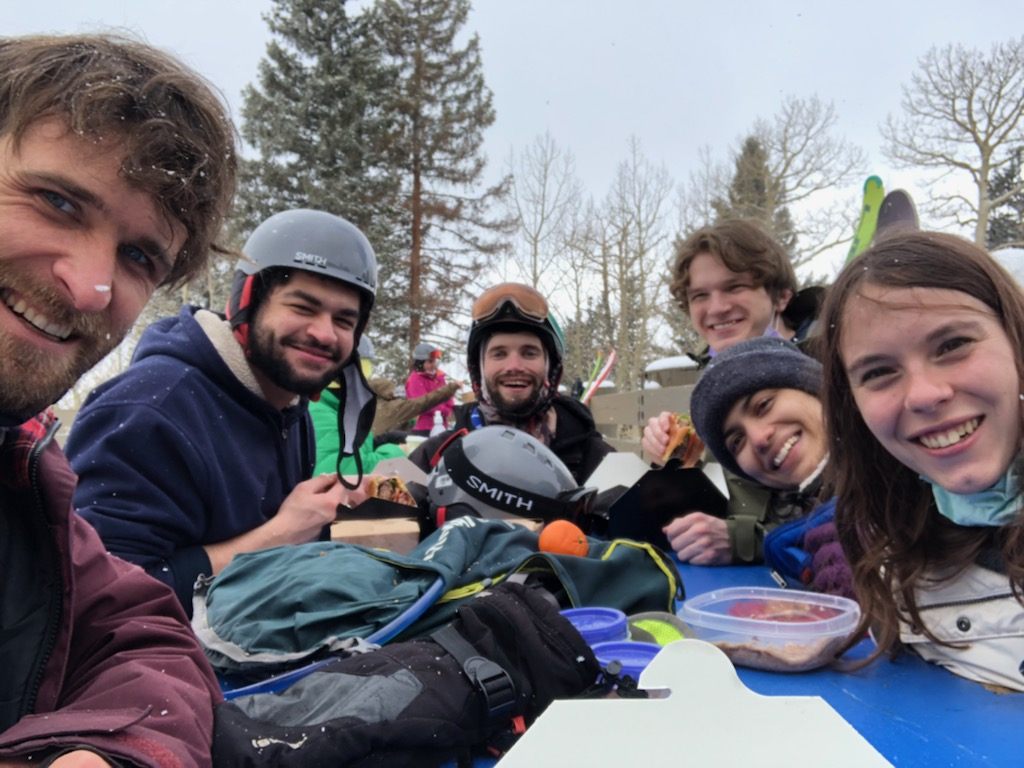
\includegraphics[height=3in]{2021-03-lab-ski-lunch} 

  Contact: toby.hocking@nau.edu

\end{frame}

\begin{frame}
  \frametitle{More notation}
  \begin{itemize}
  \item   First let $\{(
\text{fpt}
(\mathbf {\hat y})
_q, \text{fnt}
(\mathbf {\hat y})
_q,
 \tau
(\mathbf {\hat y})
_q
)\}_{q=1}^Q$ 
be a sequence of $Q$ tuples, each of which corresponds to a point on the ROC curve (and an interval on the fn/fp error plot). 
\item For each $q$ the
  $\text{fpt}(\mathbf {\hat y})_q, \text{fpt}(\mathbf {\hat y})_q$ are
  false positive/negative totals at that point (in that interval) whereas
  $\tau(\mathbf {\hat y})_q$ is the upper limit of the interval.
\item The limits are increasing, $ -\infty = \tau
(\mathbf {\hat y})
_0 < \cdots <  \tau
(\mathbf {\hat y})
_Q = \infty$.
% \item For each $q\in\{1,\dots,Q\}$ there is a corresponding interval of values $c$ between $\tau(\mathbf {\hat y})_{q-1}$ and $\tau(\mathbf {\hat y})_q$
% such that 
% $\text{FPT}_{\mathbf{\hat y}}(c)=\text{fpt}(\mathbf {\hat y})_q$
% and
% $\text{FNT}_{\mathbf{\hat y}}(c)=\text{fnt}(\mathbf {\hat y})_q$
% for all $c\in(\tau(\mathbf {\hat y})_{q-1}, \tau(\mathbf {\hat y})_q)$.
\item Then we define $m(\mathbf {\hat y})_q = \min\{
    \text{fpt}(\mathbf {\hat y})_q , \, 
    \text{fnt}(\mathbf {\hat y})_q
\}$ as the min of fp and fn totals in that interval.
  \end{itemize}

  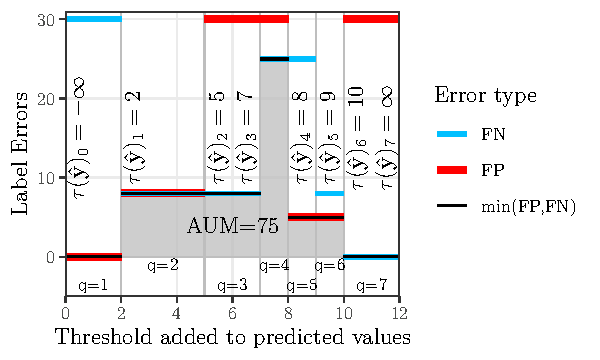
\includegraphics[height=1.5in]{figure-more-than-one-more-aum}
  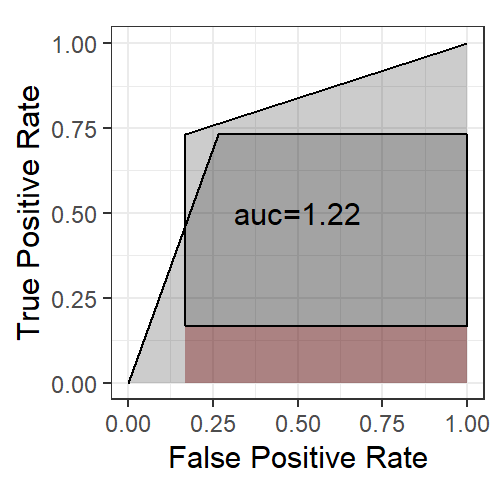
\includegraphics[height=1.5in]{figure-more-than-one-more-auc}

\end{frame}

\begin{frame}
  \frametitle{L1 relaxation interpretation}
  
Our proposed loss function is
\begin{equation*}
\label{eq:AUM-computation}
    \text{AUM}(\mathbf {\hat y}) =
    \sum_{q=2}^{Q-1}
    [ \tau(\mathbf {\hat y})_{q} - \tau(\mathbf {\hat y})_{q-1} ]
    m(\mathbf {\hat y})_q.
\end{equation*}

It is an L1 relaxation of the following non-convex \textbf{S}um of \textbf{M}in(FP,FN) function, 
\begin{equation*}
\label{eq:SM-computation}
    \text{SM}(\mathbf {\hat y}) =
    \sum_{q=2}^{Q-1}
    I[ \tau(\mathbf {\hat y})_{q} \neq \tau(\mathbf {\hat y})_{q-1} ]
    m(\mathbf {\hat y})_q =
    \sum_{q:\tau(\mathbf {\hat y})_{q} \neq \tau(\mathbf {\hat y})_{q-1} }
    m(\mathbf {\hat y})_q.
\end{equation*}

\end{frame}

\begin{frame}
  \frametitle{Definition of data set, notations}

  \begin{itemize}
  \item Let there be a total of $B$ breakpoints in the error functions over
    all $n$ labeled training examples.
  \item Each breakpoint
  $b\in\{1,\dots, B\}$ is represented by the tuple
  $(v_b, \Delta\text{FP}_b, \Delta\text{FN}_b, \mathcal I_b)$, where the
  $\mathcal I_b\in\{1,\dots,n\}$ is an example index, and there are
  changes $\Delta\text{FP}_b, \Delta\text{FN}_b$ at predicted value
  $v_b\in\mathbb R$ in the error functions.
\item For example in binary
  classification, there are $B=n$ breakpoints (same as the number of
  labeled training examples); for each breakpoint $b\in\{1,\dots,B\}$
  we have $v_b=0$ and $\mathcal I_b=b$.  For breakpoints $b$ with
  positive labels $y_b=1$ we have
  $\Delta\text{FP}=0,\Delta\text{FN}=-1$, and for negative labels
  $y_b=-1$ we have $\Delta\text{FP}=1,\Delta\text{FN}=0$.  
\item   In
  changepoint detection we have more general error functions, which
  may have more than one breakpoint per example.
  \end{itemize}
  
\end{frame}

\end{document}
